%%% -*- mode: latex; flyspell-mode: nil; -*-

\documentclass{beamer}

\mode<presentation>

\usepackage{tikz}

\begin{document}


\begin{frame}{Microstructured fiber example: Geometry}


  \begin{center}

    Geometry modeled after the paper [Francesco Poletti. Nested
    antiresonant nodeless hollow core fiber (2014)].

    \bigskip
    
    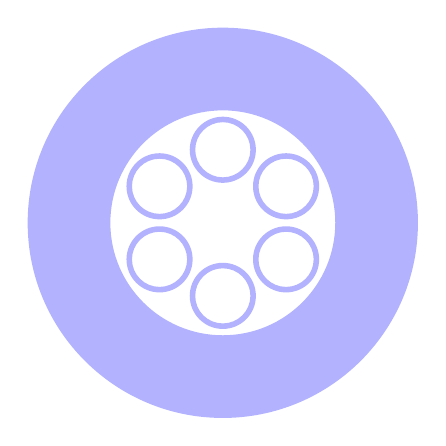
\begin{tikzpicture}[scale=0.035]

      \fill [blue!30,even odd rule] (0,0)
      circle[radius=70.8]
      circle[radius=40.8];
      
      % The north capillary tube.
      \fill [blue!30,even odd rule] (0.0, 26.505) 
      circle [radius=12]
      circle [radius=10];

      
      % The northwest tube.
      \fill [blue!30,even odd rule] (-22.954003327306545, 13.2525) 
      circle [radius=12]
      circle [radius=10];
      
      % The southwest tube.
      \fill [blue!30,even odd rule] (-22.954003327306545, -13.2525) 
      circle [radius=12]
      circle [radius=10];
      
      % The south tube.
      \fill [blue!30,even odd rule] (0.0, -26.505) 
      circle [radius=12]
      circle [radius=10];
      % \draw (0.0, -26.505) circle [radius=12];
      % \draw (0.0, -26.505) circle [radius=10];

      % The southeast tube.
      \fill [blue!30,even odd rule] (22.954003327306545, -13.2525) 
      circle [radius=12]
      circle [radius=10];
      
      % The northeast tube.
      \fill [blue!30,even odd rule] (22.954003327306545, 13.2525) 
      circle [radius=12]
      circle [radius=10];

    \end{tikzpicture}
  \end{center}
\end{frame}



\begin{frame}{Microstructured fiber example: Parameters}


    \begin{center}
    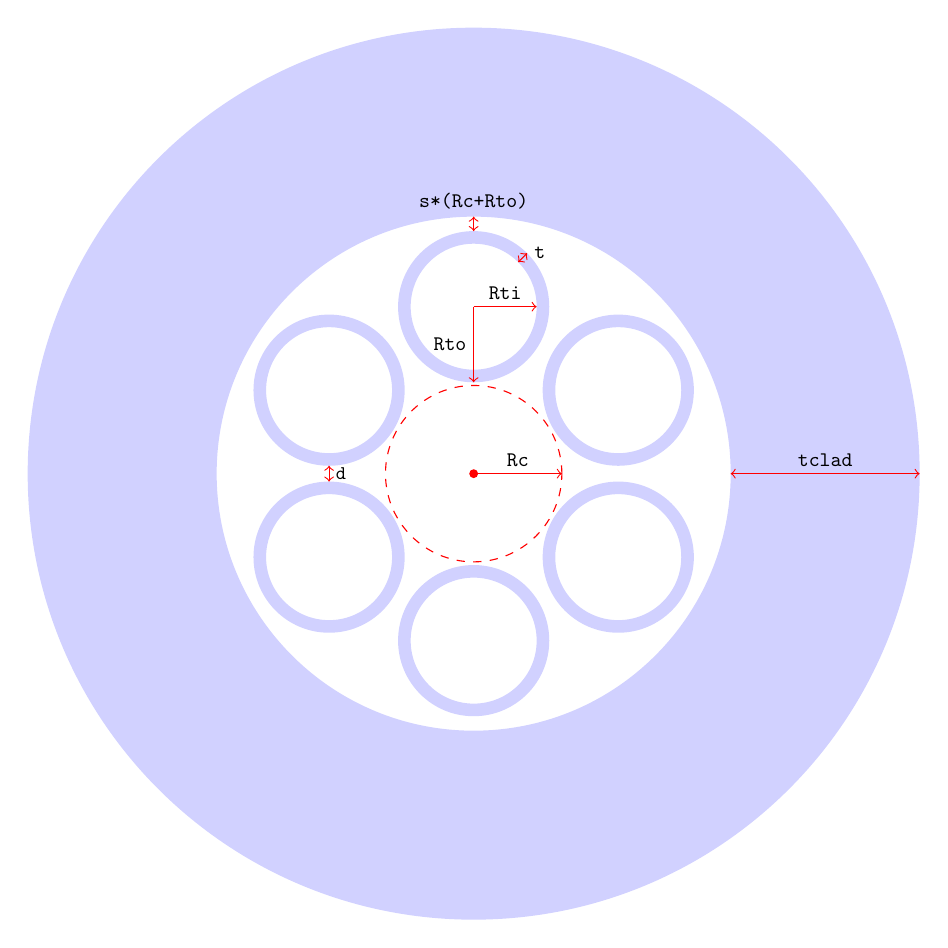
\begin{tikzpicture}[scale=0.08]

      \fill [blue!30,even odd rule,opacity=0.6] (0,0)
      circle[radius=70.8]
      circle[radius=40.8];
      
      
      % outer cladding layer
      \draw[red, <->] (40.8,0) -- (70.8,0)
      node [scale=0.75,black, midway, above] {{\tt{tclad}}};
      
            
      % The inner core region.
      \draw[red, dashed] (0,0) circle [radius=14.0];
      \draw[red, ->] (0,0) -- (14,0) node [scale=0.75,black, midway,
      above,fill=white] {{\tt{Rc}}};
      \fill[red] (0,0) circle (20pt);
            
      % The north capillary tube.
      \fill [blue!30,even odd rule,opacity=0.6] (0.0, 26.505) 
      circle [radius=12]
      circle [radius=10];
      
      % Outer and inner radius of the capillary tubes.
      \draw[red, ->] (0.0, 26.505) -- (0.0, 14.505)
      node [scale=.75, black, midway, left] {{\tt{Rto}}}; 

      \draw[->, red] (0.0, 26.505) -- (10.0, 26.505)
      node [scale=0.75, black, midway, above] {{\tt{Rti}}};
      
      % Create a label for the distance between the north capillary
      % tube and
      % the boundary of the core region.
      \draw[<->,red] (0.0, 38.505) -- (0.0, 40.8)
      node [scale=0.75, black, above] {\tt{s*(Rc+Rto)}};
      
      % Create a label for the thickness of the capillary tubes.
      \draw[red, <->] (7.071067811865475, 33.57606781186547) --
      (8.48528137423857, 34.99028137423857) node [scale=0.75, black,
      above, right] {{\tt{t}}}; % {$t$};
      
      % The northwest tube.
      \fill [blue!30,even odd rule,opacity=0.6] (-22.954003327306545, 13.2525) 
      circle [radius=12]
      circle [radius=10];
      
      % The southwest tube.
      \fill [blue!30,even odd rule,opacity=0.6] (-22.954003327306545,
      -13.2525) circle [radius=12] circle [radius=10];
      
      % A line to indicate the distance between any two capillary tubes.
      \draw[<->, red]
      (-22.954003327306545, 1.2525) -- (-22.954003327306545, -1.2525)
      node [scale=0.7, black, midway, right] {{\tt{d}}};
      
      % The south tube.
      \fill [blue!30,even odd rule,opacity=0.6] (0.0, -26.505) 
      circle [radius=12]
      circle [radius=10];

      % The southeast tube.
      \fill [blue!30,even odd rule,opacity=0.6] (22.954003327306545, -13.2525) 
      circle [radius=12]
      circle [radius=10];

      % The northeast tube.
      \fill [blue!30,even odd rule,opacity=0.6] (22.954003327306545,
      13.2525) circle [radius=12] circle [radius=10];
    \end{tikzpicture}
  \end{center}
\end{frame}


\begin{frame}{Embedded Microstructured fiber example: Parameters}


    \begin{center}
    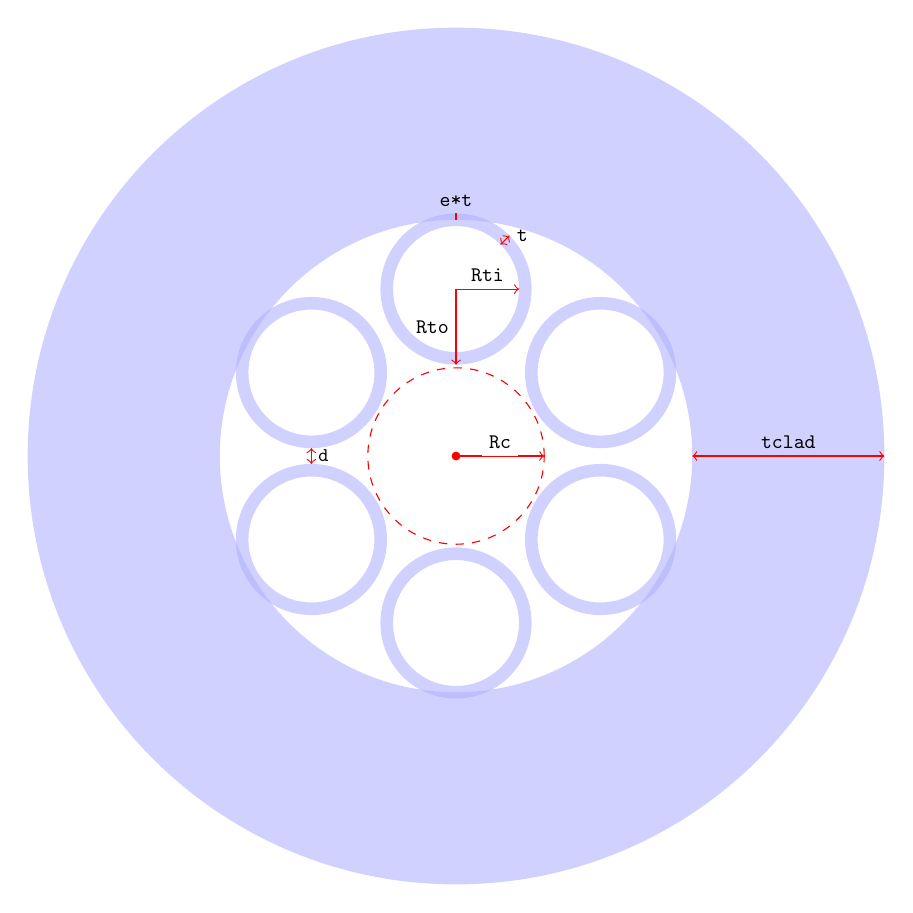
\begin{tikzpicture}[scale=0.08]

      \fill [blue!30,even odd rule,opacity=0.6] (0,0)
      circle[radius=68]
      circle[radius=37.5];
      
      
      % outer cladding layer
      \draw[red, <->] (37.5,0) -- (68,0)
      node [scale=0.75,black, midway, above] {{\tt{tclad}}};
      
            
      % The inner core region.
      \draw[red, dashed] (0,0) circle [radius=14.0];
      \draw[red, ->] (0,0) -- (14,0) node [scale=0.75,black, midway,
      above,fill=white] {{\tt{Rc}}};
      \fill[red] (0,0) circle (20pt);
            
      % The north capillary tube.
      \fill [blue!30,even odd rule,opacity=0.6] (0.0, 26.505) 
      circle [radius=12]
      circle [radius=10];
      
      % Outer and inner radius of the capillary tubes.
      \draw[red, ->] (0.0, 26.505) -- (0.0, 14.505)
      node [scale=.75, black, midway, left] {{\tt{Rto}}}; 

      \draw[->, red] (0.0, 26.505) -- (10.0, 26.505)
      node [scale=0.75, black, midway, above] {{\tt{Rti}}};
      
      % Create a label for the distance that a given capillary
      % tube is embedded into the glass jacket.
      \draw[-,red] (0.0, 37.505) -- (0.0, 38.505)
      node [scale=0.75, black, above] {\tt{e*t}};
      
      % Create a label for the thickness of the capillary tubes.
      \draw[red, <->] (7.071067811865475, 33.57606781186547) --
      (8.48528137423857, 34.99028137423857) node [scale=0.75, black,
      above, right] {{\tt{t}}}; % {$t$};
      
      % The northwest tube.
      \fill [blue!30,even odd rule,opacity=0.6] (-22.954003327306545, 13.2525) 
      circle [radius=12]
      circle [radius=10];
      
      % The southwest tube.
      \fill [blue!30,even odd rule,opacity=0.6] (-22.954003327306545,
      -13.2525) circle [radius=12] circle [radius=10];
      
      % A line to indicate the distance between any two capillary tubes.
      \draw[<->, red]
      (-22.954003327306545, 1.2525) -- (-22.954003327306545, -1.2525)
      node [scale=0.7, black, midway, right] {{\tt{d}}};
      
      % The south tube.
      \fill [blue!30,even odd rule,opacity=0.6] (0.0, -26.505) 
      circle [radius=12]
      circle [radius=10];

      % The southeast tube.
      \fill [blue!30,even odd rule,opacity=0.6] (22.954003327306545, -13.2525) 
      circle [radius=12]
      circle [radius=10];

      % The northeast tube.
      \fill [blue!30,even odd rule,opacity=0.6] (22.954003327306545,
      13.2525) circle [radius=12] circle [radius=10];
    \end{tikzpicture}
  \end{center}
\end{frame}



\begin{frame}{Embedded Microstructured fiber example: A closer look}


    \begin{center}
    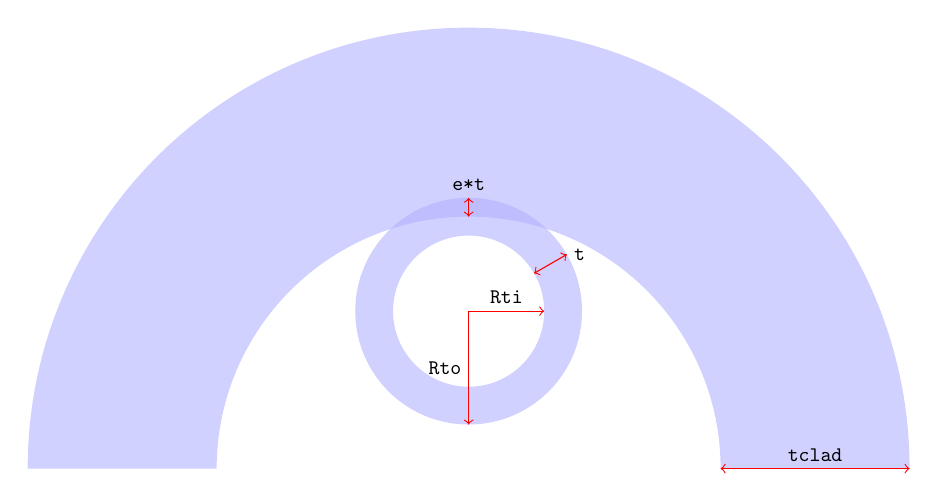
\begin{tikzpicture}[scale=0.08]

      \fill[fill=blue!30, even odd rule, opacity=0.6] (70,0)
      arc [radius=70, start angle=0, delta angle=180]
      -- (-40, 0) arc [radius=40, start angle=180, delta angle=-180]
      -- cycle;
      
      % outer cladding layer
      \draw[red, <->] (40,0) -- (70,0)
      node [scale=0.75,black, midway, above] {{\tt{tclad}}};
            
      % The north capillary tube.
      \fill [blue!30,even odd rule,opacity=0.6] (0.0, 25) 
      circle [radius=18]
      circle [radius=12];
      
      % Outer and inner radius of the capillary tubes.
      \draw[red, ->] (0.0, 25) -- (0.0, 7)
      node [scale=.75, black, midway, left] {{\tt{Rto}}}; 

      \draw[->, red] (0.0, 25) -- (12, 25)
      node [scale=0.75, black, midway, above] {{\tt{Rti}}};
      
      % Create a label for the distance that a given capillary
      % tube is embedded into the glass jacket.
      \draw[<->,red] (0.0, 40) -- (0.0, 43)
      node [scale=0.75, black, above] {\tt{e*t}};
      
      % Create a label for the thickness of the capillary tubes.
      \draw[red, <->] (10.39230485, 31.) --
      (15.58845727, 34.) node [scale=0.75, black,
      above, right] {{\tt{t}}};
    \end{tikzpicture}
  \end{center}
\end{frame}

\end{document}

%%% Local Variables:
%%% mode: latex
%%% TeX-master: t
%%% End:
